\subsection{Raw data}
This paper is based on a data set consisting of prices of the four cryptocurrencies of interest Bitcoin, Etherium, XRP and Litecoin, of the CMC Crypto 200 Index and of the 10 year US treasury bond. The data was sourced form Yahoo! through its Application Programming Interface (API). For each of the above mentioned assets, the daily (adjusted) closing price was retrieved. The data set spans from January 1, 2018 to November 12, 2022.\\

To get a feel for the data set, in Figure \ref{fig:mov_treasury} we plotted the movement of the 10 year treasury yield over the whole time span form 2018 to 2022. Analogously, in Figure \ref{fig:mov_crypto} we depicted the price movements of all the cryptocurrencies and the cryptocurrency index.

\begin{figure}[!h]
    \centering
    \caption{10 year treasury yield}
    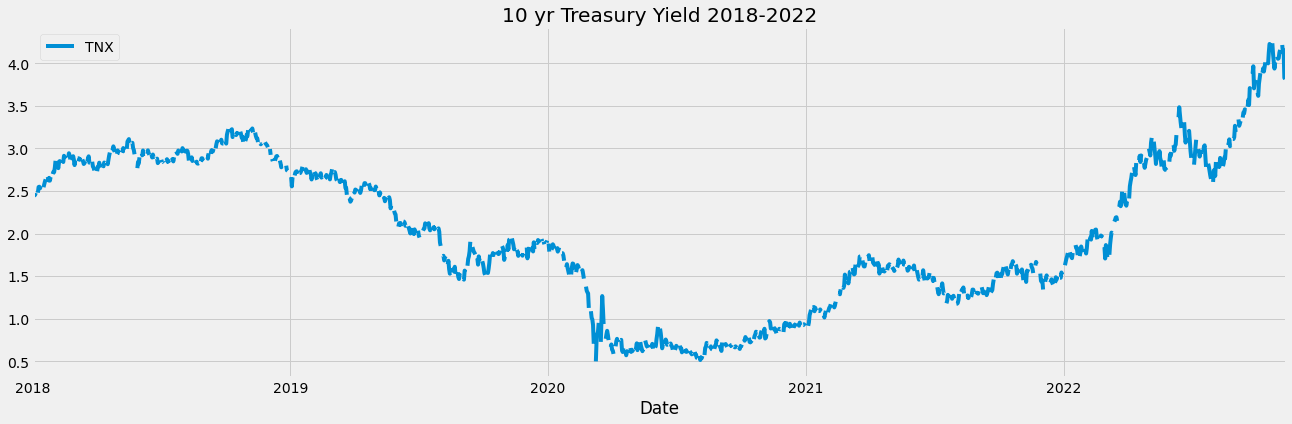
\includegraphics[width=\textwidth,height=\textheight,keepaspectratio]{images/movement_treasury.png}
    \label{fig:mov_treasury}
    \note{\textit{Note.} Own representation based on raw data set 2018-2022.}
\end{figure}

\begin{figure}[!h]
    \centering
    \caption{Price cryptocurrencies}
    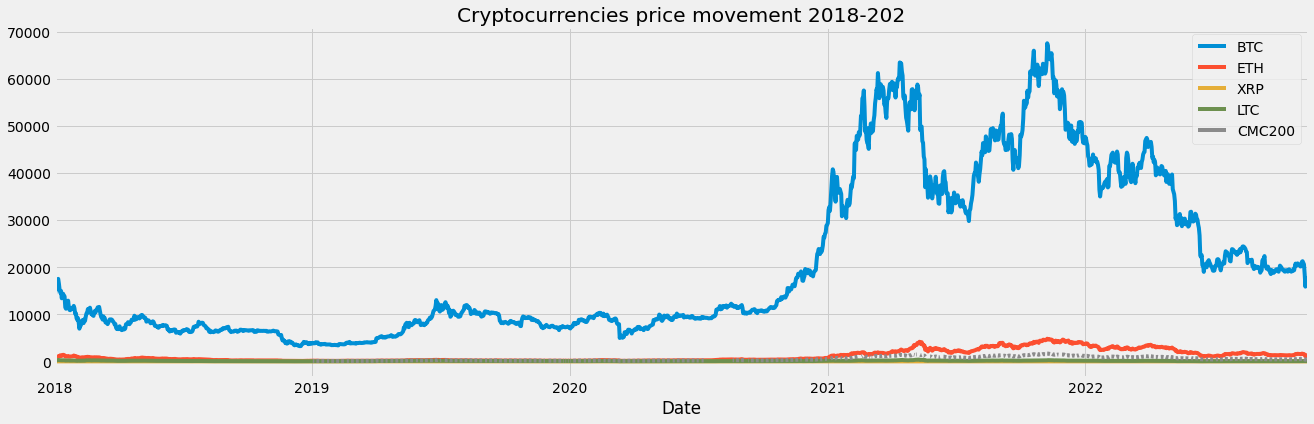
\includegraphics[width=\textwidth,height=\textheight,keepaspectratio]{images/movement_crypto.png}
    \label{fig:mov_crypto}
    \note{\textit{Note.} Own representation based on raw data set 2018-2022.}
\end{figure}

\subsection{Final data set}
As the CMC Crypto 200 Index was launched only at year end 2018, there is a lack of data with respect to the index for the first year within our sample. Therefore we decided to excluded year 2018 from our data set to avoid bias in our figures. All follwing figures and analyses will be based on this reduced time span of 4 years, from 2019-2022. We also did some cleaning the data set and replaced any NaN values with zeros.
Finally, we calculated the returns of the cryptocurrencies. These compose our final data set. The means of all variables (Figure \ref{fig:mean}) and the standard deviations (Figure \ref{fig:std}) of the cryptocurrencies. These two statistics are based on the final data set, excluding year 2018. ETH has clearly the highest closing price on average, the 10 year treasury bond (referred to as TNX) the lowest. Regarding standard deviation, XRP has the highest value.


\begin{figure}
\centering
\begin{minipage}{.5\textwidth}
  \centering
  \caption{Means}
  \label{fig:mean}
  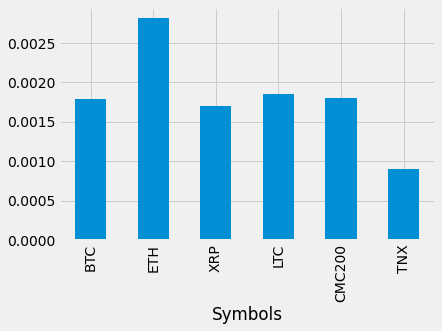
\includegraphics[height=5.8cm,keepaspectratio]{images/mean.png}
  \note{\textit{Note.} Own representation based on final data set 2019-2022.}
\end{minipage}%
\begin{minipage}{.5\textwidth}
  \centering
  \caption{Standard deviations}
  \label{fig:std}
  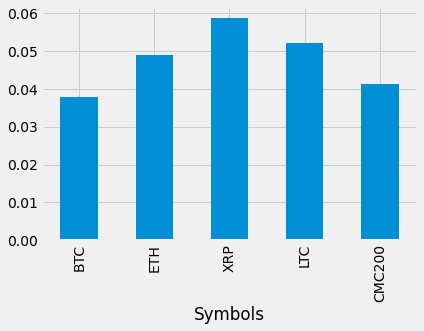
\includegraphics[height=5.8cm,keepaspectratio]{images/std.png}
  \note{\textit{Note.} Own representation based on final data set 2019-2022.}
\end{minipage}
\end{figure}

The final data set is openly accessible on our GitHub page, allowing for reproduction of our exact results:
\paragraph{Object name} data\_adjusted\_small.parquet
\paragraph{Format names and versions} Parquet
\paragraph{Creation date} 2022-11-15
\paragraph{Dataset creator} Jakob Pirs (co-author)
\paragraph{Language} English
%\paragraph{API} yahoo 
\paragraph{Repository name} GitHub 
\paragraph{Repository path} \url{https://github.com/ncanto/group-work.git}


%Here you can provide, if applicable, information about the dataset(s) whose creation, collection, management, access, processing or analysis have been discussed in this paper, following this schema:
%\paragraph{Object name} Typically the name of the file or file set in the repository.
%\paragraph{Format names and versions} E.g., ASCII, CSV, Autocad, EPS, JPEG, Excel, SQL, etc.
%\paragraph{Creation dates} The start and end dates of when the data was created (YYYY-MM-DD).
%\paragraph{Dataset creators} Please list anyone who helped to create the dataset (who may or may not be an author of the data paper), including their roles (using and affiliations).
%\paragraph{Language} Languages used in the dataset (i.e., for variable names etc.).
%\paragraph{License} The open license under which the data has been deposited (e.g., CC0). 
%\paragraph{Repository name} The name of the repository to which the data is uploaded. E.g., Figshare, Dataverse, etc. 
%\paragraph{Publication date} If already known, the date in which the dataset was published in the repository (YYYY-MM-DD).


